%!TEX root = ../ENTRUST_TR.tex
ActivFORMS is a formal approach for self-adaptation that uses an integrated formal model of the adaptive components and knowledge models. The formal model is executed directly by a virtual machine to realize adaptation, hence called active model. ActivFORMS approach distinguishes itself from existing approaches in two ways. First, the formally verified model of the complete feedback loop is directly executed by the virtual machine, which guarantees the verified adaptation goals at runtime. As the active model is directly executed by ActivFORMS, the approach does not require coding. Second, ActivFORMS supports dynamic change of the active model. A new feedback loop model can be deployed at runtime to meet new or changing goals. 

\begin{figure}[b!]
	\centering
	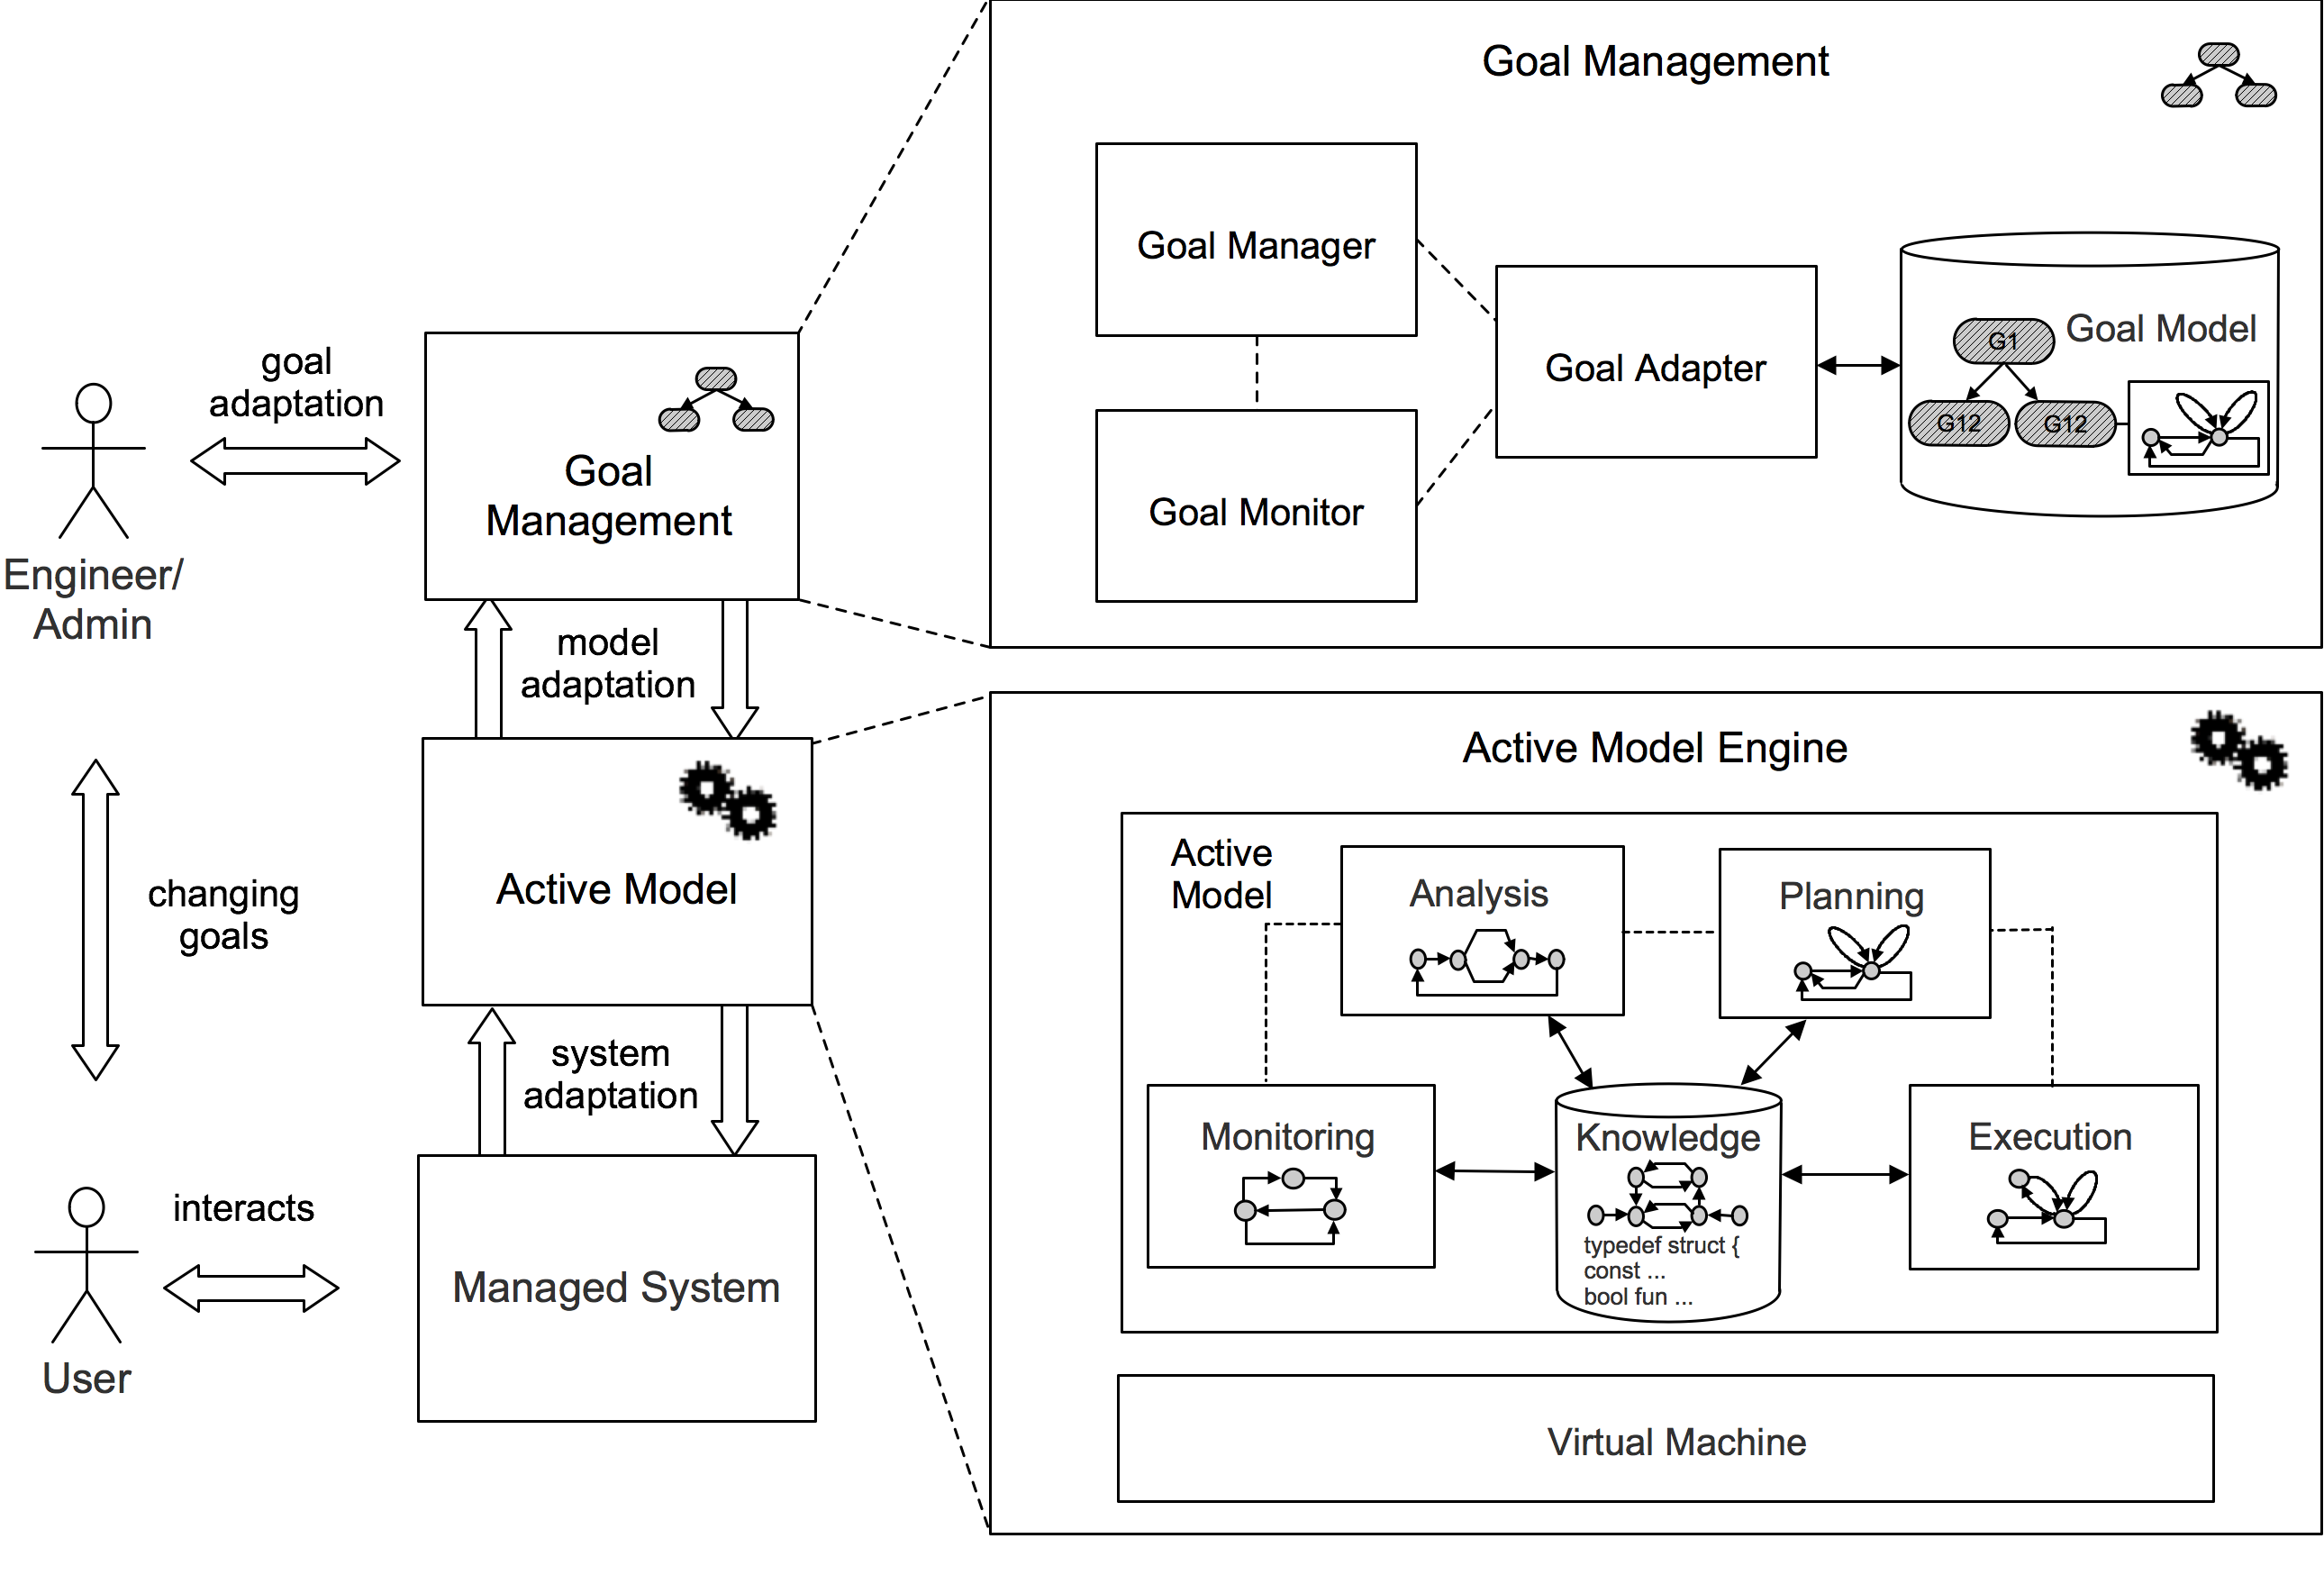
\includegraphics[width=0.7\textwidth]{figures/ActivFORMS-approach.png}
	\caption{ActivFORMS approach}\label{fig:activforms}
\end{figure}

Figure~\ref{fig:activforms} shows the primary modules of the ActivFORMS. The approach is in line with the three layered reference model for self-adaptive systems proposed by Kramer and Magee~\cite{Kramer2007:FOSE}. The managed system realizes the domain functionality for users. The active model consists of two parts: an integrated formal model that realises a feedback loop, i.e., the active model, and a virtual machine that can execute the active model. The active model monitors and adapts the managed system through probes and effectors, respectively. 

ActivFORMS supports feedback loops modelled using networks of timed automata~\cite{Alur1990}. A timed automaton is a finite-state machine that models a behaviour, extended with clock variables. Automata can synchronize through channels. There are two types of channels, binary channels and broadcast channels. For a binary channel, a sender x! can synchronize with a receiver x? through a signal. If there are multiple receivers x? then a single receiver will be chosen non-deterministically. The sender x! will be blocked if there is no receiver. On the contrary, a broadcast channel sends a signal to all the receivers, and if there is no receiver, the sender will not be blocked. Behaviour specifications can be complemented with expressions specified in a C-like language to define data structures (struct concept) and functions. Goals can be expressed in timed computation tree logic expressions (TCTL). TCTL expressions describe the state and path formulae that can be verified, such as reachability (a system should/can/cannot/... reach a particular state or set of states), liveness (something eventually will hold), etc. We use Uppaal~\cite{Behrmann2004}, a model checking tool that supports modelling of behaviours and verification of properties.

The goal management layer handles adaptation issues that cannot be performed by the current active model. The goal management consists of four parts, i.e., goal model, goal monitor, goal adapter and goal manager. The goal model represents the adaptation goals. ActivFORMS uses a AND-OR tree-based goal model to specify goals. The goals can be expressed as boolean expressions, and the goals at the bottom level of each subtree have associated models to realise adaptations. The goal monitor checks periodically the status of the goals and if any goal is violated, it notifies the goal adapter. The goal adapter is the heart of goal management. When the goal adapter receives a signal  from the goal monitor about a goal change, it consults the goal model and searches for a matching model that satisfies the changing situation. If the model associated with the changing goal differs from the currently deployed model, the goal adapter starts updating the current model with the new model at the virtual machine. If the model does not differ no further action is required. The goal manager offers support for three primary functions: inspecting the active model and its ongoing execution, monitoring and updating goals, and updating the goal model. In our current implementation, the ActivFORMS user interface connects with the goal managers of different system nodes. The user interface enables a software engineer, e.g., a system administrator, to operate the goal manager remotely.
